\documentclass{article}
\usepackage{ctex}
\usepackage{bm}
\usepackage{bbm}
\usepackage{amsmath}
\usepackage{amsthm}
\usepackage{algorithm,algorithmic}
\usepackage{url}
\usepackage{amssymb}
\usepackage{mathtools}
\usepackage{hyperref}
\usepackage{xcolor}
\newtheorem{theorem}{Theorem}
\newtheorem{example}{Example}
\newtheorem{lemma}{Lemma}
\def\E{\mathbb{E}}
\def\R{\mathbb{R}}
\DeclareMathOperator{\erf}{erf}
\title{Experimental report}
\begin{document}
\maketitle
\section{The upper bound of actual sample size}
\subsection{Cauchy distribution}
\begin{theorem}\label{thm:poly_tail_sample_complexity}
    For distributions with polynomial tails with $k>0$, given $\epsilon \in (0,1)$,
    when the following condition is satisfied
  \begin{equation}\label{eq:N_c_d_3_2}
    N = \frac{c^d}{k^{1/2}d^{3/2} \epsilon}, \textrm{ where } c=\frac{\sqrt{\pi}k\Gamma(k/2)}{\Gamma(\frac{k+1}{2})}>1  
  \end{equation}
  the interpolation error $p_{N,d} < \epsilon$ as $d\to \infty$.
  \end{theorem}
Take $\epsilon=0.5$ and the Cauchy distribution, we can obtain
the empirical $N'$ such that
$p_{N',d} = \epsilon$ and the upper bound of $N'$ by
\eqref{eq:N_c_d_3_2}. The relationship of $N-d$, $N'-d$ is shown in
Figure \ref{fig:cauchy} for $d=2,\dots, 10$.
\begin{figure}[!ht]
    \centering
    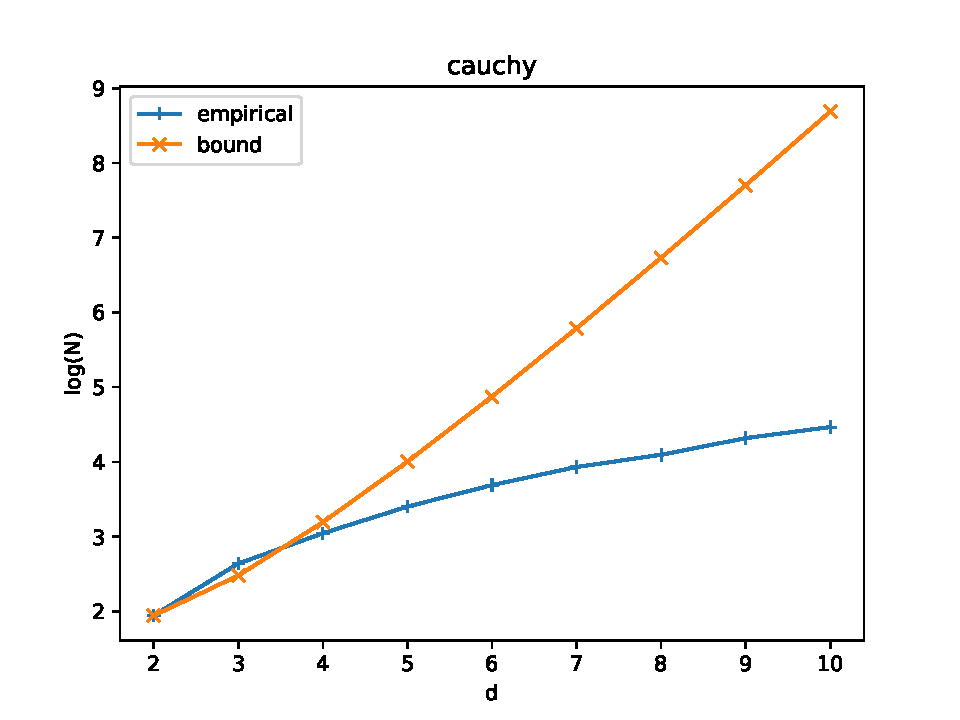
\includegraphics[width=8cm]{cauchy.pdf}
    \caption{}\label{fig:cauchy}
\end{figure}

The multivariate Cauchy distribution is a special case
of multivariate t-distribution with $\nu=1$.
Let $Y\sim N(0,I_d)$
and $U\sim \mathcal{X}_{\nu}^2$, then
$Y/\sqrt{\frac{U}{v}}$ follows the multivariate t-distribution
\cite{mtd}.
\subsection{Gaussian distribution}
\begin{theorem}\label{thm:exp_tails_sample}
    For distributions with exponential tails, given $\epsilon \in (0,1)$, when the following condition is satisfied
    \begin{equation}\label{N_d_relationship_exp_tail}
      N\cdot \gamma(N)^{(d-1)/2} = \frac{(2\pi)^{d/2} }{d^{3/2} \epsilon},
    \end{equation}
    the interpolation error $p_{N,d} < \epsilon$ as $d\to \infty$.
  \end{theorem}
For standard Gaussian distribution, we have $\gamma(N)=(2\log N)^{-1}$,
we can solve $N$ from \eqref{N_d_relationship_exp_tail} for a given $d$ to get the upper bound.
The relationship of $N-d$, $N'-d$ is shown in
Figure \ref{fig:gaussian} for $d=2,\dots, 7$.
\begin{figure}[!ht]
    \centering
    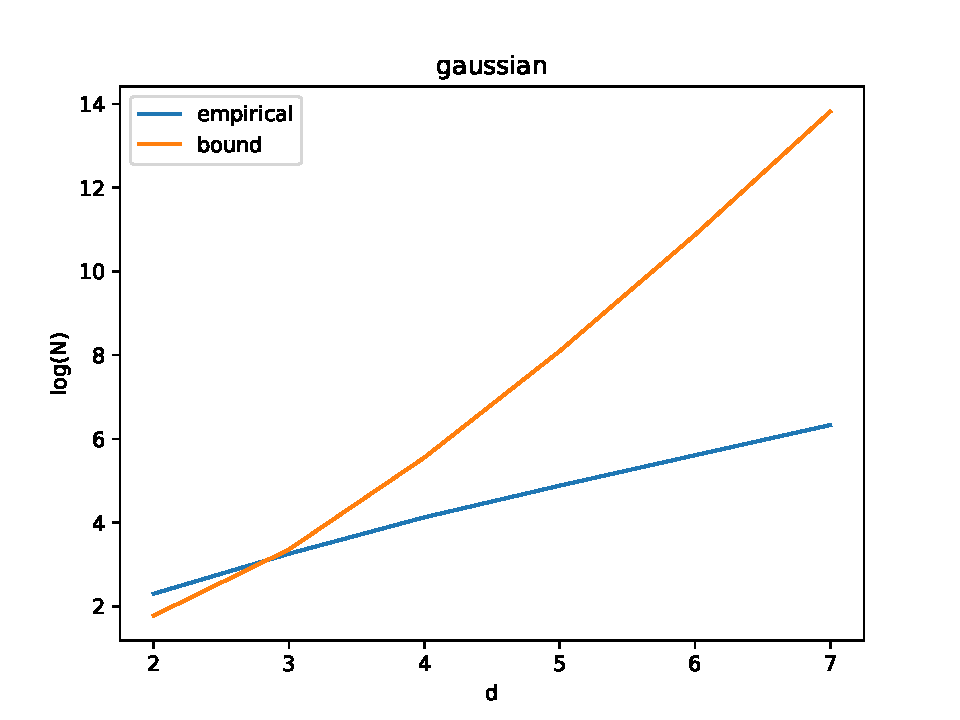
\includegraphics[width=8cm]{gaussian.pdf}
    \caption{$\epsilon=0.5$}\label{fig:gaussian}
\end{figure}
\subsection{Uniform distribution in a sphere}
\begin{theorem}\label{thm:truncated_tails_sample}
    For distributions with truncated tails,
    given $\epsilon \in (0,1)$,
    when the following condition is satisfied
    \begin{equation}\label{eq:N_truncated_tail_eps_relation}
      \frac{N^{\frac{2k}{2k+d-1}}}{L(N)^{\frac{d-1}{2k+d-1}}} 
          =\frac{(2\pi)^{d/2}d^{(d-5)/2}}{\epsilon},
    \end{equation}
    the interpolation error $p_{N,d} < \epsilon$ as $d\to \infty$.
  \end{theorem}
For uniform distribution in a sphere, $L(N)=d, k=1$,
we can solve $N$ from \eqref{eq:N_truncated_tail_eps_relation}
for a given $d$ to get the upper bound.
The relationship of $N-d$, $N'-d$ is shown in
Figure \ref{fig:uniform} for $d=2,\dots, 7$.
\begin{figure}[!ht]
    \centering
    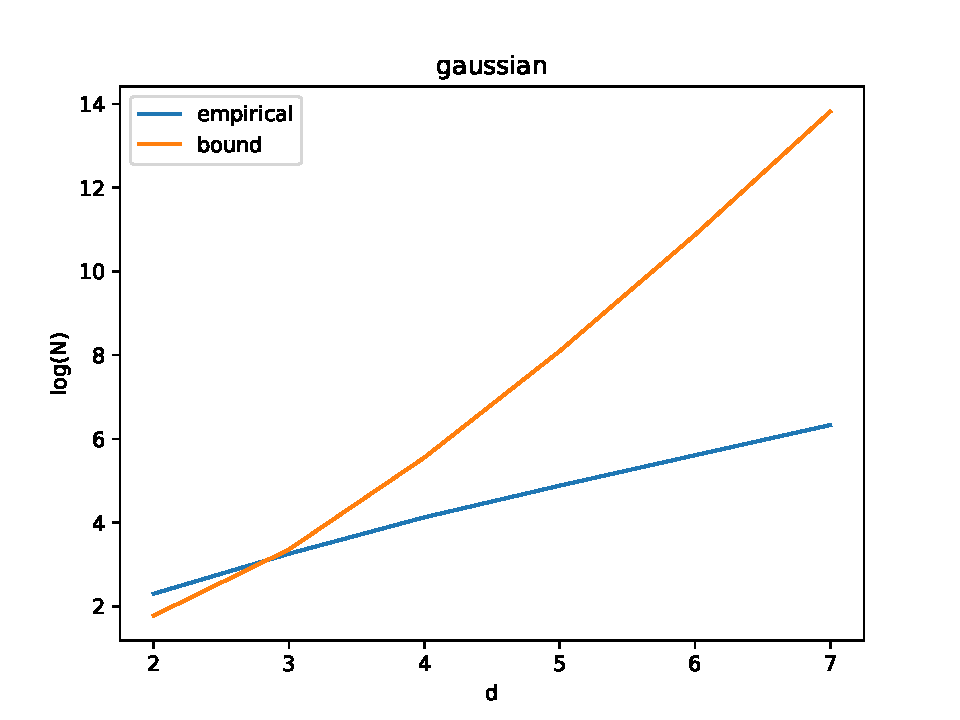
\includegraphics[width=8cm]{gaussian.pdf}
    \caption{$\epsilon=0.9$}\label{fig:uniform}
\end{figure}
In the simulation, the uniform distribution is generated by $U^{\frac{1}{d}}X$,
where $U$ is a random number chosen from the interval $[0, 1]$ and $X$ is uniform on the unit sphere.
$X$ can be generated by normalizing a Gaussian vector. That is,
\begin{equation}
    X = \frac{(X_1, \dots, X_d)}{\sqrt{X_1^2+\dots +X_d^2}}, X_i \sim \mathcal{N}(0,1)
\end{equation}

\begin{thebibliography}{9}
    \bibitem{mtd} \url{https://en.wikipedia.org/wiki/Multivariate_t-distribution}
\end{thebibliography}
\end{document}



